\documentclass[12pt, titlepage]{article}

\usepackage{booktabs}
\usepackage{tabularx}
\newcolumntype{L}[1]{>{\raggedright\let\newline\\\arraybackslash\hspace{0pt}}p{#1}}
\usepackage{hyperref}
\hypersetup{
    colorlinks,
    citecolor=blue,
    filecolor=black,
    linkcolor=red,
    urlcolor=blue
}
\usepackage[round]{natbib}

\usepackage[shortlabels]{enumitem}
\usepackage{float}
\usepackage{geometry}
\usepackage{pdflscape}
\usepackage{siunitx}
\usepackage{graphicx}

\newcommand{\rt}[1]{\textcolor{red}{#1}}


%% Comments

\usepackage{color}

\newif\ifcomments\commentstrue %displays comments
%\newif\ifcomments\commentsfalse %so that comments do not display

\ifcomments
\newcommand{\authornote}[3]{\textcolor{#1}{[#3 ---#2]}}
\newcommand{\todo}[1]{\textcolor{red}{[TODO: #1]}}
\else
\newcommand{\authornote}[3]{}
\newcommand{\todo}[1]{}
\fi

\newcommand{\wss}[1]{\authornote{blue}{SS}{#1}} 
\newcommand{\plt}[1]{\authornote{magenta}{TPLT}{#1}} %For explanation of the template
\newcommand{\an}[1]{\authornote{cyan}{Author}{#1}}

%% Common Parts

\newcommand{\progname}{SFWRENG 4G06 Capstone Design Project} % PUT YOUR PROGRAM NAME HERE
\newcommand{\projname}{MotionMingle} % project name
\newcommand{\authname}{Team \#18, InfiniView-AI
\\ Anhao Jiao
\\ Kehao Huang
\\ Qianlin Chen
\\ Shu Qi
\\ Xunzhou Ye
} % AUTHOR NAMES

\usepackage{hyperref}
    \hypersetup{colorlinks=true, linkcolor=blue, citecolor=blue, filecolor=blue,
                urlcolor=blue, unicode=false}
    \urlstyle{same}


\begin{document}

\title{Verification and Validation Report: \progname} 
\author{\authname}
\date{\today}

\maketitle

\pagenumbering{roman}

\section{Revision History}

\begin{tabularx}{\textwidth}{llX}
  \toprule {\bf Date} & {\bf Developer(s)} & {\bf Change} \\
  \midrule
Mar 6 & AJ, QS, KH, XY, QC & Initial draft \\
  \bottomrule
\end{tabularx}

\newpage

\section{Symbols, Abbreviations and Acronyms}

Table \ref{tab:abbrv} lists all the symbols, abbreviations, and acronyms used
throughout this document.
\renewcommand{\arraystretch}{1.2}
\begin{table}[H]
  \centering
  \begin{tabular}{L{0.25\linewidth}L{0.8\linewidth}} \toprule
    \textbf{Symbol}                  & \textbf{Description}                                                                                                                                                                    \\ \midrule
    Instructor                 & A person who teaches a Tai Chi class through an online conference system.                                                                                                          \\
    Performance test           & Testing the performance(includes different metrics) of a system.                                                                                                                   \\
    Pipeline                   & A sequence of processing elements connected in series, which are responsible for generating annotations.                                                                           \\
    POC                        & proof of concept.                                                                                                                                                                  \\
    Practitioner               & A person who learns Tai Chi through an online conference system.                                                                                                                   \\
    SFU                        & Selective Forwarding Unit, a component in real-time communication systems like WebRTC that routes and selectively forwards audio and video streams from one participant to others. \\
    SRS                        & The Software Requirements Specification document.                                                                                                                                  \\
    Stress test                & Testing the limits (often the amount of data) of a system.                                                                                                                         \\
    TA                         & Teaching Assistant.                                                                                                                                                                \\
    Tai Chi                    & A classical Chinese martial art system practiced for health promotion and rehabilitation.                                                                                          \\
    UI                         & User Interface.                                                                                                                                                                    \\
    V\&V Plan                  & The verification and validation plan document.                                                                                                                                     \\
    MIN\_RES \label{const:res} & 720p                                                                                                                                                                               \\ \bottomrule
  \end{tabular}
  \caption{List of symbols, abbreviations, and acronyms}
  \label{tab:abbrv}
\end{table}

\newpage

\tableofcontents

\listoftables %if appropriate

\listoffigures %if appropriate

\newpage

\pagenumbering{arabic}

This document reports the results of the verification and validation process for
MotionMingle.

\section{Functional Requirements Evaluation}

\begin{enumerate}[FR-T1]
  \item \label{FRT1}
    \begin{description}
    \item[Initial State] Client application is running on the user's device, but
      the user didn’t do any operations yet.
    \item[Input/Condition] User clicks on the applicable
      identity(instructor/practitioner) button
    \item[Expected Output] The live stream video window pops out on the user's
      screen.
    \item[Actual Output] The live stream video window shows on the instructor's
      screen, it doesn't show on the practitioner's screen.
    \item[Result] Pass
    \end{description}
  \item \label{FRT2}
    \begin{description}
    \item[Initial State] Application running on user’s computer, and the user has
      clicked on “the instructor identity button” to indicate they are a TaiChi
      instructor. A window asking for permission to use the camera on the
      instructor's device popped out.
    \item[Input/Condition] User allow/deny the webcam permission
    \item[Expected Output] The webcam on the instructor’s device is turned on
    \item[Actual Output] The webcam on the instructor’s device is turned on after
      allowing webcam permission, and the webcam is not turned on after denying
      permission.
    \item[Result] Pass
    \end{description}
  \item \label{FRT3}
    \begin{description}
    \item[Initial State] both client applications and the server are running.
    \item[Input/Condition] The user clicks on the applicable identity button to
      indicate they are an instructor or a practitioner.
    \item[Expected Output] A log message indicates connection between the user’s
      device and the server has been established.
    \item[Actual Output] Log message confirms a successful connection between the
      user’s device and the server for both instructor and practitioner.
    \item[Result] Pass
    \end{description}
  \item \label{FRT4}
    \begin{description}
    \item[Type] Functional, Dynamic, Automated
    \item[Initial State] The live stream Window for practitioners.
    \item[Input/Condition] The user’s device has established a connection with the
      server as a practitioner device.
    \item[Expected Output] A request from the client device to the server for
      accessing the list of available annotation configuration.
    \item[Actual Output] The client device sends a request to the server for the
      list of available annotation configurations.
    \item[Result] Pass
    \end{description}
  \item \label{FRT5}
    \begin{description}
    \item[Initial State] The selectable list of the type of annotations is
      rendered on the user's screen.
    \item[Input/Condition] Practitioner’s selection on the list of types of
      annotations.
    \item[Expected Output] A request(that reflects user’s annotation selection)
      from the client device to the server for updating the annotation
      configuration, with a log indicating the request is sent.
    \item[Actual Output] The client device sends the selected annotation
      configuration update to the server, and a log entry confirms the request
      was sent.
    \item[Result] Pass
    \end{description}
  \item \label{FRT6}
    \begin{description}
    \item[Initial State] The system is running and actively connected to
      practitioners.
    \item[Input/Condition] Practitioners initiate updates to annotation
      configurations.
    \item[Expected Output] The system receives and processes the updated annotation
      configurations.
    \item[Actual Output] The server gets the request and user sees the annotation
      they selected.
    \item[Result] Pass
    \end{description}
  \item \label{FRT7}
    \begin{description}
    \item[Initial State] The server is running and actively receiving annotation
      configuration updates.
    \item[Input/Condition] In a controlled test environment, the
      practitioner-client initiates the update of an annotation configuration.
      The update is sent to the server for processing.
    \item[Expected Output] The expected result is that the server correctly
      processes the received annotation configuration from the
      practitioner-client.
    \item[Actual Output] The server is not able to receive annotation configuration
      updates while the connection has been established.
    \item[Result] Fail
    \end{description}
  \item \label{FRT8}
    \begin{description}
    \item[Initial State] The server has received and processed the annotation
      configuration.
    \item[Input/Condition] The server uses the received annotation configuration to
      configure machine learning pipelines.
    \item[Expected Output] The machine learning pipelines are arranged and
      configured based on the annotation configuration.
    \item[Actual Output] The server successfully arranges and configures machine
      learning pipelines according to the received annotation configuration.
    \item[Result] Pass
    \end{description}
  \item \label{FRT9}
    \begin{description}
    \item[Initial State] The machine learning pipelines are configured and active.
    \item[Input/Condition] The instructor's video stream is processed with the
      annotation configuration.
    \item[Expected Output] The instructor's video stream is rendered with
      annotations.
    \item[Actual Output] The instructor's video stream is processed with the
      annotations.
    \item[Result] Pass
    \end{description}
  \item \label{FRT10}
    \begin{description}
    \item[Initial State] The server is actively connected to practitioner clients.
    \item[Input/Condition] The annotated video stream is generated and ready for
      transmission.
    \item[Expected Output] The annotated video stream is transmitted to each
      practitioner-client through their established connections.
    \item[Actual Output] The annotated video stream is transmitted to practitioner
      clients.
    \item[Result] Pass
    \end{description}
  \item \label{FRT11}
    \begin{description}
    \item[Initial State] The signaling server is running.
    \item[Input/Condition] Signaling requests for WebRTC connections are initiated.
    \item[Expected Output] The signaling server consistently responds to requests
      and establishes WebRTC connections.
    \item[Actual Output] The signaling server responds to most requests and
      establishes WebRTC connections
    \item[Result] Pass
    \end{description}
  \item \label{FRT12}
    \begin{description}
    \item[Initial State] The client application is running, but the user didn’t do
      any operations yet
    \item[Input/Condition] The user joining video stream session.
    \item[Expected Output] A button to identify if a user is an instructor or a
      practitioner is rendered.
    \item[Actual Output] The button to identify a user as an instructor or a
      practitioner is rendered without issues
    \item[Result] Pass
    \end{description}
  \end{enumerate}

\section{Nonfunctional Requirements Evaluation}

\begin{enumerate}[NFR-T1]
  \item \label{NFRT1}
    \begin{description}
    \item[Initial State] The system is in a typical operational state with all
      components and services running, including the user interface.
    \item[Input/Condition] User interactions such as button clicks and menu
      selections.
    \item[Expected Output] The user is able to interact with the client application
      and understand the response from and results yielded by the system.
    \item[Actual Output] All 5 users are able to successfully interact with the
      application with understandable responses and results from the system.
    \item[Result] Pass
    \end{description}
  \item \label{NFRT2}
    \begin{description}
    \item[Initial State] The system is in a typical operational state with all
      components and services running, including the user interface.
    \item[Input/Condition] User interactions such as button clicks and menu
      selections.
    \item[Expected Output] System response to user interactions.
    \item[Actual Output] The system responds to user interactions promptly and
      correctly.
    \item[Result] Pass
    \end{description}
  \item \label{NFRT3}
    \begin{description}
    \item[Initial State] The system is in a stable operational state with necessary
      services and components active. No users are currently logged in.
    \item[Input/Condition] 5 test accounts (or more) for users. Predefined user
      actions/scripts (relevant to normal system interactions during peak
      periods).
    \item[Expected Output] The system remains stable and responsive. All user
      transactions are processed successfully.
    \item[Actual Output] The system remains stable and responsive with all user
      transactions processed successfully. This is evident in the survey result
      part 3 in figure \ref{fig:surveyp3}.
    \item[Result] Pass
    \end{description}
  \item \label{NFRT4}
    \begin{description}
    \item[Initial State] The system is operational, with all services and
      components running. User accounts for test are set up, and no tasks are
      being performed.
    \item[Input/Condition] Erroneous user input data. Improper user actions.
    \item[Expected Output] The system detects and rejects invalid inputs or
      actions, providing clear and helpful error messages to the user.
      Transactions or actions are either rolled back safely or do not proceed
      until valid input is provided.
    \item[Actual Output] No invalid inputs can be made within the system.
    \item[Result] Pass
    \end{description}
  \stepcounter{enumi}
  \item \label{NFRT6}
    \begin{description}
    \item[Initial State] The system, with the SFU component, is in a stable,
      operational state. Initially, there is a base number of video streams
      being processed, which is within the SFU's current capacity.
    \item[Input/Condition] A load testing tool or custom script capable of
      simulating multiple, simultaneous video streams.
    \item[Expected Output] The SFU successfully processes an increasing number of
      video streams.
    \item[Actual Output] The SFU processes an increased number of video streams,
      which was up to 5 users without significant issues.
    \item[Result] Pass
    \end{description}
  \item \label{NFRT7}
    \begin{description}
    \item[Initial State] This system is in a typical operational state with all
      components and services running, the user is in a live session.
    \item[Input/Condition] Network Interruption/Network Resumption
    \item[Expected Output] The system attempts to resume the previous session.
    \item[Actual Output] The system did not resume to the previous session.
    \item[Result] Fail
    \end{description}
  \item \label{NFRT8}
    \begin{description}
    \item[Initial State] This system is in a typical operational state with all
      components and services running, the user is in a live session.
    \item[Input/Condition] Network instability
    \item[Expected Output] A pop up window for network instability warning.
    \item[Actual Output] There was no pop up window for network instability
      warning.
    \item[Result] Fail
    \end{description}
  \item \label{NFRT9}
    \begin{description}
    \item[Initial State] This system is in a typical operational state with all
      components and services running.
    \item[Input/Condition] Turn down the primary signaling server.
    \item[Expected Output] The redundant server takes over until the primary server
      resumes.
    \item[Actual Output] Connections were able to be established without the
      primary signaling server.
    \item[Result] Pass
    \end{description}
  \item \label{NFRT10}
    \begin{description}
    \item[Initial State] The system is in a typical operational state with all
      components and services running. The user is in a live session with a
      media capturing device plugged in.
    \item[Input/Condition] Disconnect the media capturing device from the user’s
      computing device.
    \item[Expected Output] A pop up window which warns the user that the client
      application has lost connection to the media capturing device and prompts
      the user to reconnect the device to resume the live session.
    \item[Actual Output] When the media capturing device is disconnected, a pop-up
      window alerts the user and prompts for reconnection.
    \item[Result] Pass
    \end{description}
  \item \label{NFRT11}
    \begin{description}
    \item[Initial State] The system is in a typical operational state with all
      components and services running.
    \item[Input/Condition] Connect a media capturing device to the user’s computing
      device.
    \item[Expected Output] A pop up window which warns the user that the video
      capturing device does not meet required specification if the client
      application detects that the video input stream has a resolution lower
      than \hyperref[const:res]{MIN\_RES}.
    \item[Actual Output] The system was not able to check the specification of the
      capturing device
    \item[Result] Fail
    \end{description}
  \item \label{NFRT12}
    \begin{description}
    \item[Initial State] The system is in a typical operational state with all
      components and services running.
    \item[Input/Condition] the user starts a live session and begins streaming.
    \item[Expected Output] Accurate instructional annotations are rendered and
      overlaid on the instructor’s video stream.
    \item[Actual Output] The system renders accurate instructional annotations on
      the instructor’s video stream.
    \item[Result] Pass
    \end{description}
  \item \label{NFRT13}
    \begin{description}
    \item[Initial State] The system is in a typical operational state with all
      components and services running.
    \item[Input/Condition] Connect more than one media capturing device to the
      user’s computing device.
    \item[Expected Output] A dialog listing all the detected capturing devices is
      displayed to prompt the user for selecting a device to use.
    \item[Actual Output] Feature handled by external API.
    \item[Result] Pass
    \end{description}
  \item \label{NFRT14}
    \begin{description}
    \item[Initial State] This system is in a typical operational state with all
      components and services running, with a live session created.
    \item[Input/Condition] The live video and audio stream from instructor client
      application.
    \item[Expected Output] Audio stream and video stream with annotations on
      practitioner client application.
    \item[Actual Output] The practitioner client application receives only video
      streams with annotations.
    \item[Result] Fail
    \end{description}
  \item \label{NFRT15}
    \begin{description}
    \item[Initial State] The system is in a typical operational state with all
      components and services running.
    \item[Input/Condition] The user starts the client application for instructors.
    \item[Expected Output] A message with detailed instruction to set up a media
      capturing device and a list of cautions is displayed.
    \item[Actual Output] No message was displayed.
    \item[Result] Fail
    \end{description}
  \item \label{NFRT16}
    \begin{description}
    \item[Initial State] The software system is fully developed, stable, and ready
      for testing. The different test environments for the latest versions of
      Windows, Linux, and macOS are set up, each with default settings.
    \item[Input/Condition] The latest stable versions of Windows, Linux, and
      macOS. Test cases designed to cover all the main functionalities of the
      system.
    \item[Expected Output] The system functions correctly on all mentioned
      operating systems without crashes, unexpected behaviour, or significant
      performance issues.
    \item[Actual Output] The system functions correctly on all mentioned operating
      systems without any significant issues.
    \item[Result] Pass \\
    \rt{ Evidence to support this result is in Survey Result \ref{fig:surveyp3}, 7 out of 10 users rated the speed and responsiveness are 5. }
    \end{description}
  \item \label{NFRT17}
    \begin{description}
    \item[Initial State] The system is fully developed, with all features
      operational, and is hosted in a stable environment accessible via the web.
      Test environments with the latest versions of Chrome, Firefox, Safari, and
      Edge are established, each configured with default browser settings.
    \item[Input/Condition] Latest stable versions of Chrome, Firefox, Safari, and
      Edge. A series of test cases designed to fully evaluate the
      functionalities and features of the system.
    \item[Expected Output] The system operates as intended on all tested web
      browsers without significant functionality issues, crashes, or severe
      performance degradation. Features and visual elements are consistent across
      all browsers.
    \item[Actual Output] The system operates as intended across all tested web
      browsers with consistent features and visual elements.
    \item[Result] Pass
    \end{description}
  \item \label{NFRT18}
    \begin{description}
    \item[Initial State] The system is fully developed and operational. The testing
      environments represent a range of standard personal computer and laptop
      configurations (covering various manufacturers, system specifications, and
      age of devices) equipped with cameras and, where applicable, microphones.
      The devices are running compatible operating systems with the necessary
      drivers installed.
    \item[Input/Condition] Range of standard computers or laptops with various
      specifications, but all within the commonly accepted 'standard' range for
      current users. Devices have functional cameras and optional microphones.
      Test script detailing system operation tasks.
    \item[Expected Output] The system operates without significant delays, errors,
      or crashes.
    \item[Actual Output] The system operates without significant delays, errors, or
      crashes across a range of standard computers and laptops.
    \item[Result] Pass
    \end{description}
  \item \label{NFRT19}
    \begin{description}
    \item[Initial State] The system is fully developed, with comprehensive
      documentation on its architecture, codebase, dependencies, and update
      procedures. The development environment is available for testing
      maintenance procedures, including tools for version control, testing, and
      deployment.
    \item[Expected Output] Successful completion of maintenance tasks without
      introducing significant issues or disruptions to the system's operation.
    \item[Actual Output] It is impossible to perform maintenance without
      interrupting live users.
    \item[Result] Fail
    \end{description}
  \addtocounter{enumi}{2}
  \item \label{NFRT22}
    \begin{description}
    \item[Initial State] The system is in a stable state, ready for testing. The
      user interface for account creation or any other information input is
      accessible, and documentation related to data handling is available.
    \item[Input/Condition] Guidelines or criteria specifying what constitutes
      "essential" versus "nonessential" information for the system’s purpose.
      Access to the system's user interfaces (UI) where data submission forms
      are present.
    \item[Expected Output] Comparison of requested data against the criteria for
      essential information.
    \item[Actual Output] The system requests only essential information from users.
    \item[Result] Pass
    \end{description}
  \item \label{NFRT23}
    \begin{description}
    \item[Initial State] This system is in a typical operational state with all
      components and services running.
    \item[Input/Condition] Attempted unauthorized modifications to the system
      including access to system files and modifications to system
      configurations.
    \item[Expected Output] A determination of whether the system are able to
      prevent access or modifications from unauthorized users.
    \item[Actual Output] The system prevents all unauthorized access and
      modifications during the test.
    \item[Result] Pass
    \end{description}
  \item \label{NFRT24}
    \begin{description}
    \item[Initial State] The system is in a typical operational state with all
      components and services running.
    \item[Input/Condition] The user starts a live session and begins streaming.
    \item[Expected Output] A prompt for granting access to use the media capturing
      devices is displayed.
    \item[Actual Output] A prompt appears for granting access to media capturing
      devices during a live session. This is evident in the survey result
      part 4 in figure \ref{fig:surveyp4}.
    \item[Result] Pass \\
    \rt{ evidence to support this result is in \ref{fig:surveyp4}, prompts appears for granting access to media captureing devices and when the instructor stops broadcasting}
    \end{description}
  \item \label{NFRT25}
    \begin{description}
    \item[Initial State] The system is in a typical operational state with all
      components and services running.
    \item[Input/Condition] The user starts a live session and begins streaming.
    \item[Expected Output] An indicator that the media capturing device is in use
      and that the user is being recorded is visible in the client application.
    \item[Actual Output] An indicator is visible in the client application when the
      media capturing device is in use.
    \item[Result] Pass
    \end{description}
  \item \label{NFRT26}
    \begin{description}
    \item[Initial State] The system is in a typical operational state with all
      components and services running.
    \item[Input/Condition] The user ends a live session and stops streaming.
    \item[Expected Output] The indicator that the media capturing device is in use
      disappears. The media stream from the capturing device is no longer
      displayed on the screen.
    \item[Actual Output] The indicator disappears, and the media stream is no
      longer displayed once the session ends.
    \item[Result] Pass
    \end{description}
  \item \label{NFRT27}
    \begin{description}
    \item[Initial State] This system is in a typical operational state with all
      components and services running.
    \item[Input/Condition] User inputs
    \item[Expected Output] System response to user inputs
    \item[Actual Output] The system responds effectively to user inputs.
    \item[Result] Pass
    \end{description}
  \item \label{NFRT28}
    \begin{description}
    \item[Initial State] The system is in a typical operational state with all
      components and services running.
    \item[Input/Condition] A set of ISO/IEC 12207 standards.
    \item[Expected Output] A determination of whether the system and its associated
      processes, documentation, and activities comply with the ISO/IEC 12207
      standards.
    \item[Actual Output] The system and its processes comply with ISO/IEC 12207
      standards as determined through evaluation.
    \item[Result] Pass
    \end{description}
  \item \label{NFRT29}
    \begin{description}
    \item[Initial State] This system is in a typical operational state with all
      components and services running.
    \item[Input/Condition] Various user interactions.
    \item[Expected Output] The computers continue to function within acceptable
      performance parameters throughout the test.
    \item[Actual Output] The computer's function is not affected throughout various
      user interactions.
    \item[Result] Pass \\
    \rt{ Evidence to support this result is in Survey Result \ref{fig:surveyp3}, 7 out of 10 users rated the speed and responsiveness are 5. }
    \end{description}
  \item \label{NFRT30}
    \begin{description}
    \item[Initial State] This system is in a typical operational state with all
      components and services running.
    \item[Input/Condition] User inputs
    \item[Expected Output] System response from user inputs
    \item[Actual Output] The system responds appropriately and efficiently to user
      inputs.
    \item[Result] Pass
    \end{description}
  \end{enumerate}

\section{Comparison to Existing Implementation}

Our project shares similarities with two existing types of implementations. The
first is a project developed by a group of researchers, focused on annotating
Tai Chi videos with detailed features such as skeletal outlines and semantic
segmentation. Like their summer Tai Chi annotation initiative, our project also
annotates videos. However, ours operates in real-time, unlike the Tai Chi
project which processes annotations offline, making ours more adept for live
online learning contexts.

Additionally, our project parallels certain aspects of video conferencing tools
like Zoom, which offer live annotation capabilities. While Zoom boasts a broader
set of features due to its maturity as a platform, our project distinguishes
itself in several key areas:

It is designed for one-directional streaming, in contrast to Zoom's
multi-directional video conferencing. Unlike Zoom, where annotations are
generated client-side, our project renders annotations server-side, minimizing
the hardware demands on viewers' devices. Our system allows viewers the
flexibility to choose their annotations, diverging from Zoom's model where
annotations are unified for all viewers as determined by the video sender. These
distinctions underscore our project's unique contributions to video annotation
technology, especially in educational and collaborative online environments.

\section{Unit Testing}
\subsection{User Authentication Module}
\begin{enumerate}[UT-UA1]
\item \label{UT-UA1}
  \begin{description}
  \item[Test Name] test\_renders\_auth\_component
  \item[Initial State] The system initializes the Auth component within a mock
    routing environment.
  \item[Input/Condition] N/A
  \item[Expected Output] The component should display the Motion Mingle banner
    and a logo image.
  \item[Actual Output] The component displayed the Motion Mingle banner and a
    logo image.
  \item[Result] Pass
  \end{description}
\item \label{UT-UA2}
  \begin{description}
  \item[Test Name] test\_instructor\_button
  \item[Initial State] The system initializes the "Auth" component within a mock
    routing environment.
  \item[Input/Condition] The user clicks on the Instructor button.
  \item[Expected Output] The user should be navigated to the '/instructor' path.
  \item[Actual Output] The user was navigated to the '/instructor' path.
  \item[Result] Pass
  \end{description}
\item \label{UT-UA3}
  \begin{description}
  \item[Test Name] test\_practitioner\_button
  \item[Initial State] The system initializes the "Auth" component within a mock
    routing environment.
  \item[Input/Condition] The user clicks on the Practitioner button.
  \item[Expected Output] The user should be navigated to the '/practitioner'
    path.
  \item[Actual Output] The user was navigated to the '/practitioner' path.
  \item[Result] Pass
  \end{description}
\item \label{UT-UA4}
  \begin{description}
  \item[Test Name] test\_slogan
  \item[Initial State] The system initializes the "Auth" component within a mock
    routing environment.
  \item[Input/Condition] N/A
  \item[Expected Output] The slogan should be visible within the component with
    the correct text.
  \item[Actual Output] The slogan was displayed within the component with the
    correct text.
  \item[Result] Pass
  \end{description}
\end{enumerate}

\subsection{Instructor View Module}
\begin{enumerate}[UT-M1]
\item \label{UT-M1}
  \begin{description}
  \item[Test Name] test\_renders\_instructor\_component
  \item[Initial State] The system is initialized with default state settings.
    The "Instructor" component is about to be rendered within a mock routing
    environment.
  \item[Input/Condition] N/A
  \item[Expected Output] The "Instructor" component should be rendered with the
    title "Motion Mingle".
  \item[Actual Output] The "Instructor" component was rendered with the title
    "Motion Mingle".
  \item[Result] Pass
  \end{description}
\item \label{UT-M2}
  \begin{description}
  \item[Test Name] test\_select\_annotation
  \item[Initial State] The system has loaded the Instructor component, and the
    "SelectAnnotation" component is ready to receive user input.
  \item[Input/Condition] A user selects "Skeleton" annotation from the dropdown
    menu.
  \item[Expected Output] The dropdown menu should reflect that "Annotation 1"
    has been selected.
  \item[Actual Output] "Skeleton" has been selected from the dropdown menu.
  \item[Result] Pass
  \end{description}
\item \label{UT-M3}
  \begin{description}
  \item[Test Name] test\_stop\_broadcast
  \item[Initial State] The Instructor component is rendered and operational,
    presumed to be in a state where broadcasting is occurring (mocked
    condition).
  \item[Input/Condition] The user clicks the "Broadcast" button to simulate
    starting a broadcast and then clicks "Stop" to simulate ending the
    broadcast.
  \item[Expected Output] The "MessageModal" mock should be displayed, indicating
    that the stopping of the video is to be confirmed.
  \item[Actual Output] The "MessageModal" mock was displayed.
  \item[Result] Pass
  \end{description}
\item \label{UT-M4}
  \begin{description}
  \item[Test Name] test\_start\_self\_video
  \item[Initial State] The Instructor component is rendered and operational. The
    self-video is initially off.
  \item[Input/Condition] The user clicks "Start self video" to initiate the
    video stream.
  \item[Expected Output] The system should transition to a state where the
    self-video is active.
  \item[Actual Output] The system transitioned to a state where the self-video
    is active.
  \item[Result] Pass
  \end{description}
\item \label{UT-M5}
  \begin{description}
  \item[Test Name] test\_close\_self\_video
  \item[Initial State] The Instructor component is rendered and operational. The
    self-video is active.
  \item[Input/Condition] The user clicks "Close self video".
  \item[Expected Output] The system should transition to a state where the
    self-video is inactive.
  \item[Actual Output] The system transitioned to a state where the self-video
    is inactive.
  \item[Result] Pass
  \end{description}
\end{enumerate}

\subsection{Practitioner View Module}
\begin{enumerate}[UT-PV1]
\item \label{UT-PV1}
  \begin{description}
  \item[Test Name] test\_renders\_practitioner\_component
  \item[Initial State] The system is initialized with default state settings.
    The "Practitioner" component is about to be rendered within a mock routing
    environment.
  \item[Input/Condition] N/A
  \item[Expected Output] The "Practitioner" component should be rendered with
    the title "Motion Mingle", a dropdown for selecting annotations initialized
    to "None", and a "Connect" button.
  \item[Actual Output] The "Practitioner" component was rendered with the title
    "Motion Mingle".
  \item[Result] Pass
  \end{description}
\item \label{UT-PV2}
  \begin{description}
  \item[Test Name] test\_select\_annotation
  \item[Initial State] The "Practitioner" component is rendered and displayed
    with the default selected annotation as "None".
  \item[Input/Condition] The user changes the annotation selection from "None"
    to "Skeleton" using the dropdown.
  \item[Expected Output] The dropdown menu for selecting annotations should
    reflect the change by displaying "Skeleton" as the current selection.
  \item[Actual Output] "Skeleton" was displayed as selected in the dropdown
    menu.
  \item[Result] Pass
  \end{description}
\item \label{UT-PV3}
  \begin{description}
  \item[Test Name] test\_start\_video\_stream
  \item[Initial State] The "Practitioner" component is rendered, displaying the
    "Connect" button while the video stream is not connected.
  \item[Input/Condition] The "Connect" button was clicked to start the video
    stream.
  \item[Expected Output] The "Connect" button should change to "Disconnect".
  \item[Actual Output] The "Connect" button changed to "Disconnect".
  \item[Result] Pass
  \end{description}
\item \label{UT-PV4}
  \begin{description}
  \item[Test Name] test\_stop\_video\_stream
  \item[Initial State] The "Practitioner" component is rendered, displaying the
    "Disconnect" button while the video stream is connected.
  \item[Input/Condition] The "Disconnect" button was clicked to stop the video
    stream.
  \item[Expected Output] The "Disconnect" button should change to "Connect".
  \item[Actual Output] The "Disconnect" button changed to "Connect".
  \item[Result] Pass
  \end{description}
\end{enumerate}

\subsection{Annotation Configuration Module}
\begin{enumerate}[UT-AC1]
\item \label{UT-AC1}
  \begin{description}
  \item[Test Name] test\_render\_select\_annotation\_component
  \item[Initial State] The "SelectAnnotation" component is initialized with
    default state settings.
  \item[Input/Condition] The component is rendered without any preselected
    value.
  \item[Expected Output] The component should display with the label
    "Annotation" and a dropdown button showing the default value "None".
  \item[Actual Output] The component was rendered with the label "Annotation"
    and a dropdown button showing the default value "None".
  \item[Result] Pass
  \end{description}
\item \label{UT-AC2}
  \begin{description}
  \item[Test Name] test\_annotation\_options
  \item[Initial State] The "SelectAnnotation" component is rendered with default
    settings.
  \item[Input/Condition] The user clicks on the dropdown menu to view available
    options.
  \item[Expected Output] The dropdown menu should display four options: "None",
    "Skeleton", "Edges", and "Cartoon".
  \item[Actual Output] The dropdown menu displayed four options: "None",
    "Skeleton", "Edges", and "Cartoon".
  \item[Result] Pass
  \end{description}
\end{enumerate}

\subsection{RTC Control Module}
\begin{enumerate}[UT-RC1]
\item \label{UT-RC1}
  \begin{description}
  \item[Test Name] test\_create\_peer\_connection
  \item[Initial State] Before creating a new "RTCPeerConnection", no connection
    exists.
  \item[Input/Condition] The "createPeerConnection" function is called without
    any specific arguments since it uses predefined settings within its
    implementation.
  \item[Expected Output] A new "RTCPeerConnection" should be created with the
    configuration specified for unified-plan SDP semantics and the Google STUN
    server.
  \item[Actual Output] A new "RTCPeerConnection" was created with the
    configuration specified for unified-plan SDP semantics and the Google STUN
    server.
  \item[Result] Pass
  \end{description}
\item \label{UT-RC2}
  \begin{description}
  \item[Test Name] test\_connect\_as\_consumer
  \item[Initial State] A "RTCPeerConnection" instance exists but has not yet
    established a connection nor created any offers.
  \item[Input/Condition] The function "connectAsConsumer" is called with the
    created peer connection and "annotation" as arguments.
  \item[Expected Output] The function should asynchronously create an SDP offer,
    set it as the local description, send it to the server, and set the received
    SDP answer as the remote description.
  \item[Actual Output] Same as expected output.
  \item[Result] Pass
  \end{description}
\item \label{UT-RC3}
  \begin{description}
  \item[Test Name] test\_connect\_as\_broadcaster
  \item[Initial State] A "RTCPeerConnection" instance is ready but not yet in a
    broadcasting state.
  \item[Input/Condition] The function "connectAsBroadcaster" is called with the
    peer connection object.
  \item[Expected Output] The function should asynchronously create an SDP offer
    for broadcasting, set it as the local description, send it to the server,
    and set the server's SDP answer as the remote description.
  \item[Actual Output] Same as expected.
  \item[Result] Pass
  \end{description}
\end{enumerate}

\subsection{Other Modules}
\begin{enumerate}[UT-OT1]
\item \label{UT-OT1}
  \begin{description}
  \item[Test Name] test\_display\_message
  \item[Initial State] The system initializes the "NotFound" component within a
    mock routing environment.
  \item[Input/Condition] The component is rendered without any user interaction.
  \item[Expected Output] The component should display the "Not Found" message.
  \item[Actual Output] The component displayed the "Not Found" message.
  \item[Result] Pass
  \end{description}
\item \label{UT-OT2}
  \begin{description}
  \item[Test Name] test\_navigate\_to\_root
  \item[Initial State] The system initializes the "NotFound" component within a
    mock routing environment.
  \item[Input/Condition] The component is rendered, and the existence of a link
    is checked.
  \item[Expected Output] There should be a link that reads "GO HOME" and
    navigates to the root path '/' upon clicking.
  \item[Actual Output] Same as expected.
  \item[Result] Pass
  \end{description}
\item \label{UT-OT3}
  \begin{description}
  \item[Test Name] test\_close\_message\_modal
  \item[Initial State] The "MessageModal" component is rendered with
    "isModalOpen" set to true.
  \item[Input/Condition] The "Cancel" button was clicked.
  \item[Expected Output] The "handleClose" mock function should be called once.
  \item[Actual Output] The "handleClose" mock function was called once.
  \item[Result] Pass
  \end{description}
\item \label{UT-OT4}
  \begin{description}
  \item[Test Name] test\_stop\_video
  \item[Initial State] The "MessageModal" component is rendered with
    "isModalOpen" set to true.
  \item[Input/Condition] The "Stop Video" button was clicked.
  \item[Expected Output] The "handelStopVideo" mock function should be called
    once.
  \item[Actual Output] The "handelStopVideo" mock function was called once.
  \item[Result] Pass
  \end{description}
\item \label{UT-OT5}
  \begin{description}
  \item[Test Name] test\_message\_visible
  \item[Initial State] The "MessageModal" component is initialized and rendered
    with "isModalOpen" set to true.
  \item[Input/Condition] N/A
  \item[Expected Output] The modal, including the warning message, should be
    visible.
  \item[Actual Output] The modal, including the warning message, was visible.
  \item[Result] Pass
  \end{description}
\item \label{UT-OT6}
  \begin{description}
  \item[Test Name] test\_message\_invisible
  \item[Initial State] The "MessageModal" component is initialized and rendered
    with "isModalOpen" set to false.
  \item[Input/Condition] N/A
  \item[Expected Output] None of the modal's content should be present in the
    document.
  \item[Actual Output] None of the modal's content was present in the document.
  \item[Result] Pass
  \end{description}
\end{enumerate}

\subsection{SFU Server Module}
\begin{enumerate}[UT-S1]
\item \label{UT-S1}
  \begin{description}
  \item[Test Name] test\_broadcast\_options
  \item[Initial State] Server is initialized and running with /broadcast
    endpoint available.
  \item[Input/Condition] HTTP OPTIONS request to /broadcast.
  \item[Expected Output] HTTP status code 200.
  \item[Actual Output] HTTP status code 200.
  \item[Result] Pass
  \end{description}

\item \label{UT-S2}
  \begin{description}
  \item[Test Name] test\_broadcast\_post
  \item[Initial State] Server is initialized with the /broadcast endpoint ready
    to accept POST requests.
  \item[Input/Condition] POST request to /broadcast with JSON body containing
    "sdp" and "type" fields.
  \item[Expected Output] HTTP status code 200 and a JSON response containing
    "sdp" and "type".
  \item[Actual Output] HTTP status code 200 and a JSON response containing "sdp"
    and "type".
  \item[Result] Pass
  \end{description}

\item \label{UT-S3}
  \begin{description}
  \item[Test Name] test\_broadcast\_empty\_body\_post
  \item[Initial State] Server is initialized with the /broadcast endpoint ready
    to accept POST requests.
  \item[Input/Condition] POST request to /broadcast with an empty JSON body.
  \item[Expected Output] HTTP status code 400
  \item[Actual Output] HTTP status code 400
  \item[Result] Pass
  \end{description}

\item \label{UT-S4}
  \begin{description}
  \item[Test Name] test\_broadcast\_post\_with\_invalid\_data\_types
  \item[Initial State] Server is initialized with the /broadcast endpoint ready.
  \item[Input/Condition] POST request to /broadcast with invalid data types for
    "sdp" and "type".
  \item[Expected Output] HTTP status code 400
  \item[Actual Output] HTTP status code 400
  \item[Result] Pass
  \end{description}

\item \label{UT-S5}
  \begin{description}
  \item[Test Name] test\_broadcast\_post\_missing\_fields
  \item[Initial State] Server is initialized with the /broadcast endpoint ready.
  \item[Input/Condition] POST request to /broadcast with missing "type" field in
    the JSON body.
  \item[Expected Output] HTTP status code 400
  \item[Actual Output] HTTP status code 400
  \item[Result] Pass
  \end{description}

\item \label{UT-S6}
  \begin{description}
  \item[Test Name] test\_invalid\_content\_type
  \item[Initial State] Server is initialized and ready to handle requests.
  \item[Input/Condition] POST request to /broadcast with a "Content-Type" of
    "text/plain".
  \item[Expected Output] HTTP status code 500
  \item[Actual Output] HTTP status code 500
  \item[Result] Pass
  \end{description}

\item \label{UT-S7}
  \begin{description}
  \item[Test Name] test\_method\_not\_allowed
  \item[Initial State] Server is initialized with the /broadcast endpoint not
    configured to accept GET requests.
  \item[Input/Condition] GET request to /broadcast.
  \item[Expected Output] HTTP status code 405
  \item[Actual Output] HTTP status code 405
  \item[Result] Pass
  \end{description}

\item \label{UT-S8}
  \begin{description}
  \item[Test Name] test\_response\_content\_type
  \item[Initial State] Server is initialized and ready to respond to POST
    requests.
  \item[Input/Condition] HTTP status code 200 and the "Content-Type" header is
    "application/json; charset=utf-8"
  \item[Actual Output] HTTP status code 200 and the "Content-Type" header is
    "application/json; charset=utf-8"
  \item[Result] Pass
  \end{description}

\item \label{UT-S9}
  \begin{description}
  \item[Test Name] test\_consume\_options
  \item[Initial State] Server is initialized and running with /consumer endpoint
    available.
  \item[Input/Condition] HTTP OPTIONS request to /consumer.
  \item[Expected Output] HTTP status code 200
  \item[Actual Output] HTTP status code 200
  \item[Result] Pass
  \end{description}

\item \label{UT-S10}
  \begin{description}
  \item[Test Name] test\_consume\_post
  \item[Initial State] Server is initialized with the /consumer endpoint ready
    to accept POST requests.
  \item[Input/Condition] POST request to /consumer with JSON body containing
    "sdp", "type", and "video\_transform".
  \item[Expected Output] HTTP status code 500
  \item[Actual Output] HTTP status code 500
  \item[Result] Pass
  \end{description}

\item \label{UT-S11}
  \begin{description}
  \item[Test Name] test\_consume\_empty\_body\_post
  \item[Initial State] Server is initialized with the /consumer endpoint ready.
  \item[Input/Condition] POST request to /consumer with an empty JSON body.
  \item[Expected Output] HTTP status code 400
  \item[Actual Output] HTTP status code 400
  \item[Result] Pass
  \end{description}

\item \label{UT-S12}
  \begin{description}
  \item[Test Name] test\_consume\_post\_unsupported\_video\_transform
  \item[Initial State] Server is initialized with the /consumer endpoint ready.
  \item[Input/Condition] POST request to /consumer with unsupported
    "video\_transform" value.
  \item[Expected Output] HTTP status code 400
  \item[Actual Output] HTTP status code 400
  \item[Result] Pass
  \end{description}
\end{enumerate}

\subsection{Video Transform Module}

Unit testing the video transform module is particularly challenging due to the
nature of its operations which involve real-time video stream manipulation using
complex image processing and machine learning models. These transformations,
such as pose estimation and segmentation, rely on the input data's visual
content, which can have near-infinite variability and require a visual context
to determine correctness. The output is highly dependent on the specific content
of the video frame being processed and the environmental conditions at the time
of capture. Furthermore, such processes are typically non-deterministic due to
the internal state management within the machine learning models (like
MediaPipe's pose detection) and can be affected by the hardware acceleration
capabilities of the environment where the tests are run.

Moreover, the transformations performed on video frames are designed to yield
results that are subjectively evaluated visually, rather than through
quantitative measures that could be programmatically asserted. While some
aspects of the module could be unit tested by mocking dependencies and checking
if the correct methods are called with expected arguments, the actual
verification of the transformation's quality requires manual inspection or more
sophisticated automated image comparison techniques that go beyond the scope of
traditional unit testing. This inherent complexity and the need for a subjective
assessment make the creation of automated unit tests for the video transform
module both non-trivial and possibly less effective for ensuring the correctness
of visual outputs.

\section{Changes Due to Testing}

\subsection{Change due to supervisor's feedback}

Andrew Mitchell, who is one of the supervisors of this project, has pointed out
during the Revision 0 demo that the “check annotated video” button on the
instructor page should appear after the instructor has started broadcasting
instead of showing it directly, as clicking the check annotated video can’t show
anything without input video stream. To follow the feedback from Andrew, the UI
design will be changed so that the “check annotated video” button only shows up
after the instructor starts broadcasting, and extra instructions will be added
to the side of the instructor and practitioner view page.

\subsection{Change due to reviewing the question in the usability survey}

The VnV Plan, states that our group will review the questions in the usability
survey as part of non-functional testing. One of the questions in the usability
survey is: “Are there any specific content or learning materials you would like
to see added to the application?” Some users state it is not convenient that
they need to manually disconnect and reconnect to the server when selecting
different annotations as a practitioner. \rt{This is stated in the question in Usability 
Survey part \ref{fig:surveyp2}: ``Are there any specific issues or challenges you've 
encountered while using the application?" The team decided to add an “auto-refresh” 
functionality to the system when an instructor or a practitioner changes their 
selected annotation. This change would make the UI more intuitive and enhance
user experiences. Another issue we observed but user didn't state in the survey: some 
users accidentally clicked the check annotated video button before starting broadcasting, 
and it led to their confusion as the remote video stream did not show. We think having 
the Check annotated video button disabled before the instructor starts broadcasting is 
a good way to avoid this confusion. To make things more clear, we also plan to add an 
instruction for users to navigate. Furthermore, we got some requests to add an annotation 
to indicate the instructor's motion on their feet in Usability Survey part \ref{fig:surveyp5}. 
We decided this is a "good to have" feature for user experience enhancement, but this 
is truly something that can make our product unique. }

\subsection{Change due to failed tests}

The VnV testing highlighted critical failures in server update processing and
network resilience. Specifically, test case \ref{FRT7} failed because the server
could not receive annotation configuration updates while the connection was
established. Additionally, the system did not handle network interruptions and
resumptions as expected in test case \ref{NFRT7}, and it also failed to provide
audio in the live video and audio streams in test case \ref{NFRT14}.

In response to these failures, the team will prioritize the development of an
'auto-reconnect' feature that ensures the system maintains or promptly
re-establishes its connection to allow continuous update processing. This
functionality will be designed to automatically resume the session and process
updates without user intervention in case of network disruptions.

For the audio issue identified in test case \ref{NFRT14}, a feature addition is
required. The team will integrate a reliable audio streaming capability to
ensure both audio and video streams are consistently received and properly
annotated in the practitioner client application.

The necessity of displaying instructional messages as indicated by the failure
of test case \ref{NFRT15} will also be addressed. The system will be updated to
show detailed instructions and cautions when starting the client application,
thereby avoiding confusion and potential misuse.

These enhancements are crucial for improving the robustness, user experience,
and functional completeness of the system. The adjustments made from these test
failures will be documented and incorporated into the VnV Plan for future
reference and to guide subsequent development cycles. The team will establish a
rigorous testing procedure for these new features to ensure their effectiveness
before deployment.

\section{Automated Testing}

\subsection{Github Action}

Github Action provides a seamless and efficient way to ensure code integrity
with each push. Tests are executed automatically on the latest commits to the
main and develop branches, verifying that new changes do not break existing
functionality.

\subsection{Pytest}
PyTest is also used for the automatic testing. It is a robust and feature-rich
Python library that streamlines the creation of test cases. By design, PyTest
simplifies test authoring, allowing developers to write test functions that are
concise and readable. It leverages the straightforward "assert" statement to
check for expected outcomes, making test assertions both natural and easy to
understand. Furthermore, PyTest's powerful parameterization capability,
facilitated by the pytest.mark.parametrize decorator, permits the execution of a
single test function against a variety of input sets. This not only enhances
test coverage but also significantly boosts efficiency, as it allows for
extensive testing without the need to write additional test cases. Overall,
Pytest's intuitive approach and its ability to facilitate detailed and
comprehensive testing with minimal code make it an invaluable tool for automated
testing, contributing to faster development cycles and more reliable software.

\section{Trace to Requirements}

\setlength{\tabcolsep}{2pt}
\newgeometry{margin=2cm}
\begin{landscape}
  \begin{table}[h!]
    \centering
    \begin{tabular}{|c|c|c|c|c|c|c|c|c|c|c|c|c|c|c|c|c|} \hline
               & FR1 & FR2 & FR3 & FR4 & FR5 & FR6 & FR7 & FR8 & FR9 & FR10 & FR11 & FR12 & FR13 & FR14 & FR15 & FR16 \\ \hline
      \ref{FRT1}  & X   & X   &     &     &     &     &     &     &     &      &      &      &      &      &      &      \\ \hline
      \ref{FRT2}  &     &     & X   &     &     &     &     &     &     &      &      &      &      &      &      & X    \\ \hline
      \ref{FRT3}  &     &     &     & X   & X   &     &     &     &     &      &      &      &      &      &      &      \\ \hline
      \ref{FRT4}  &     &     &     &     &     & X   &     &     &     &      &      &      &      &      & X    &      \\ \hline
      \ref{FRT5}  &     &     &     &     &     &     &     & X   &     &      &      &      &      &      &      &      \\ \hline
      \ref{FRT6}  &     &     &     &     &     &     & X   &     &     &      &      &      &      &      &      &      \\ \hline
      \ref{FRT7}  &     &     &     &     &     &     &     &     & X   &      &      &      &      &      &      &      \\ \hline
      \ref{FRT8}  &     &     &     &     &     &     &     &     &     & X    &      &      &      &      &      &      \\ \hline
      \ref{FRT9}  &     &     &     &     &     &     &     &     &     &      & X    &      &      &      &      &      \\ \hline
      \ref{FRT10} &     &     &     &     &     &     &     &     &     &      &      & X    &      &      &      &      \\ \hline
      \ref{FRT11} &     &     &     &     &     &     &     &     &     &      &      &      & X    &      &      &      \\ \hline
      \ref{FRT12} &     &     &     &     &     &     &     &     &     &      &      &      &      & X    &      &      \\ \hline
    \end{tabular}
    \caption{Traceability matrix showing the connections between test cases
      and functional requirements}
    \label{tab:frt}
  \end{table}
  \begin{table}[h!]
    \centering
    \begin{tabular}{|c|c|c|c|c|c|c|c|c|c|c|c|c|c|c|c|c|} \hline
                & LF1 & UH1 & UH2 & PR1 & PR2 & PR3 & PR4 & PR5 & PR6 & PR7 & PR8 & PR9 & PR10 & PR11 & PR12 & PR13 \\ \hline
      \ref{NFRT1}  & X   & X   & X   &     &     &     &     &     &     &     &     &     &      &      &      &      \\ \hline
      \ref{NFRT2}  &     &     &     & X   & X   &     &     &     &     &     &     &     &      &      &      &      \\ \hline
      \ref{NFRT3}  &     &     &     &     & X   & X   &     &     &     &     &     &     &      &      &      &      \\ \hline
      \ref{NFRT4}  &     &     &     &     &     &     & X   &     &     &     &     &     &      &      &      &      \\ \hline
      \ref{NFRT6}  &     &     &     &     &     &     &     &     & X   &     &     &     &      &      &      &      \\ \hline
      \ref{NFRT7}  &     &     &     &     &     &     &     &     &     & X   &     &     &      &      &      &      \\ \hline
      \ref{NFRT8}  &     &     &     &     &     &     &     &     &     &     & X   &     &      &      &      &      \\ \hline
      \ref{NFRT9}  &     &     &     &     &     &     &     &     &     &     &     & X   &      &      &      &      \\ \hline
      \ref{NFRT10} &     &     &     &     &     &     &     &     &     &     &     &     & X    &      &      &      \\ \hline
      \ref{NFRT11} &     &     &     &     &     &     &     &     &     &     &     &     &      & X    &      &      \\ \hline
      \ref{NFRT12} &     &     &     &     &     &     &     &     &     &     &     &     &      &      & X    &      \\ \hline
      \ref{NFRT13} &     &     &     &     &     &     &     &     &     &     &     &     &      &      &      & X    \\ \hline
    \end{tabular}
    \caption{Traceability matrix showing the connections between test cases
      and non-functional requirements}
    \label{tab:nfrt1}
  \end{table}
  \begin{table}[h!]
    \centering
    \begin{tabular}{|c|c|c|c|c|c|c|c|c|c|c|c|c|c|c|c|c|c|} \hline
                & PR14 & PR15 & OE1 & OE2 & OE3 & MS1 & MS2 & SR1 & SR2 & SR3 & SR4 & SR5 & SR6 & CR1 & LR1 & HS1 & HS2 \\ \hline
      \ref{NFRT14} & X    &      &     &     &     &     &     &     &     &     &     &     &     &     &     &     &     \\ \hline
      \ref{NFRT15} &      & X    &     &     &     &     &     &     &     &     &     &     &     &     &     &     &     \\ \hline
      \ref{NFRT16} &      &      & X   &     &     &     &     &     &     &     &     &     &     &     &     &     &     \\ \hline
      \ref{NFRT17} &      &      &     & X   &     &     &     &     &     &     &     &     &     &     &     &     &     \\ \hline
      \ref{NFRT18} &      &      &     &     & X   &     &     &     &     &     &     &     &     &     &     &     &     \\ \hline
      \ref{NFRT19} &      &      &     &     &     & X   &     &     &     &     &     &     &     &     &     &     &     \\ \hline
      \ref{NFRT22} &      &      &     &     &     &     &     &     & X   &     &     &     &     &     &     &     &     \\ \hline
      \ref{NFRT23} &      &      &     &     &     &     &     &     &     & X   &     &     &     &     &     &     &     \\ \hline
      \ref{NFRT24} &      &      &     &     &     &     &     &     &     &     & X   &     &     &     &     &     &     \\ \hline
      \ref{NFRT25} &      &      &     &     &     &     &     &     &     &     &     & X   &     &     &     &     &     \\ \hline
      \ref{NFRT26} &      &      &     &     &     &     &     &     &     &     &     &     & X   &     &     &     &     \\ \hline
      \ref{NFRT27} &      &      &     &     &     &     &     &     &     &     &     &     &     & X   &     &     &     \\ \hline
      \ref{NFRT28} &      &      &     &     &     &     &     &     &     &     &     &     &     &     & X   &     &     \\ \hline
      \ref{NFRT29} &      &      &     &     &     &     &     &     &     &     &     &     &     &     &     & X   &     \\ \hline
      \ref{NFRT30} &      &      &     &     &     &     &     &     &     &     &     &     &     &     &     &     & X   \\ \hline
    \end{tabular}
    \caption{Traceability matrix showing the connections between test cases
      and non-functional requirements continued}
    \label{tab:nfrt2}
  \end{table}
\end{landscape}
\restoregeometry

\section{Trace to Modules}
\begin{landscape}
  \begin{table}[h!]
    \centering
    \label{tab:traceability_matrix}
    \small 
    \setlength\tabcolsep{4pt}
    \renewcommand{\arraystretch}{1.2}
    \begin{tabular}{|c|*{10}{c|}}
      \hline
      & \rotatebox{90}{User Authentication Module} & \rotatebox{90}{Instructor View Module} & \rotatebox{90}{Practitioner View Module} & \rotatebox{90}{Annotation Configuration Module} & \rotatebox{90}{RTC Control Module} & \rotatebox{90}{STUN Server Module} & \rotatebox{90}{App Module} & \rotatebox{90}{Video Transform Module} & \rotatebox{90}{Human Pose Estimation Module} & \rotatebox{90}{SFU Server Module} \\ \hline
      FR-T1 &   & X &   &   &   &   & X &   &   &   \\ \hline
      FR-T2 & X & X &   &   &   &   &   &   &   &   \\ \hline
      FR-T3 &   &   &   &   & X & X &   &   &   &   \\ \hline
      FR-T4 &   &   & X & X &   &   &   &   &   &   \\ \hline
      FR-T5 &   &   & X & X &   &   &   &   &   &   \\ \hline
      FR-T6 &   &   & X & X &   &   &   &   &   &   \\ \hline
      FR-T7 &   &   & X & X &   &   &   &   &   &   \\ \hline
      FR-T8 &   &   &   & X &   &   &   &   & X &   \\ \hline
      FR-T9 &   & X &   &   &   &   &   & X &   &   \\ \hline
      FR-T10 &  &   & X &   &   &   &   & X &   & X \\ \hline
      FR-T11 &  &   &   &   & X & X &   &   &   &   \\ \hline
      FR-T12 & X & X & X &   &   &   & X &   &   &   \\ \hline
      \end{tabular}
    \caption{Traceability matrix showing the connections between functional requirement test cases and modules}
  \end{table}

  \begin{table}[ht]
    \centering
    \label{tab:traceability_nfr}
    \begin{tabular}{|l|*{10}{c|}} % Adjust the number of columns as needed
    \hline
    & \rotatebox{90}{User Authentication Module} & \rotatebox{90}{Instructor View Module} & \rotatebox{90}{Practitioner View Module} & \rotatebox{90}{Annotation Configuration Module} & \rotatebox{90}{RTC Control Module} & \rotatebox{90}{STUN Server Module} & \rotatebox{90}{App Module} & \rotatebox{90}{Video Transform Module} & \rotatebox{90}{Human Pose Estimation Module} & \rotatebox{90}{SFU Server Module} \\ \hline
    NFR-T1 & X & X & X &   &   &   & X &   &   &   \\ \hline
    NFR-T2 &   &   &   &   & X & X &   &   &   &   \\ \hline
    NFR-T3 &   &   &   &   & X & X &   &   &   & X \\ \hline
    NFR-T4 & X & X & X & X & X & X & X & X & X & X \\ \hline
    NFR-T6 &   &   &   &   &   &   &   &   &   & X \\ \hline
    NFR-T7 &   &   &   &   & X & X &   &   &   &   \\ \hline
    NFR-T8 &   &   &   &   & X & X &   &   &   &   \\ \hline
    NFR-T9 &   &   &   &   & X & X &   &   &   &   \\ \hline
    NFR-T10 &  &   &   &   &   &   & X & X &   &   \\ \hline
    NFR-T11 &  &   &   &   &   &   & X & X &   &   \\ \hline
    NFR-T12 &  &   &   &   &   &   &   & X & X &   \\ \hline
    NFR-T13 &  &   &   &   &   &   & X &   &   &   \\ \hline
    NFR-T14 &  &   &   &   &   &   &   & X &   &   \\ \hline
    NFR-T15 &  &   &   &   &   &   & X &   &   &   \\ \hline
    \end{tabular}
    \caption{Traceability Matrix showing the connections between Non-Functional Requirements and Modules}
  \end{table}
  
  \begin{table}[ht]
    \centering
    \label{tab:traceability_nfr}
    \begin{tabular}{|l|*{10}{c|}} % Adjust the number of columns as needed
    \hline
    & \rotatebox{90}{User Authentication Module} & \rotatebox{90}{Instructor View Module} & \rotatebox{90}{Practitioner View Module} & \rotatebox{90}{Annotation Configuration Module} & \rotatebox{90}{RTC Control Module} & \rotatebox{90}{STUN Server Module} & \rotatebox{90}{App Module} & \rotatebox{90}{Video Transform Module} & \rotatebox{90}{Human Pose Estimation Module} & \rotatebox{90}{SFU Server Module} \\ \hline
    NFR-T16 &  &   &   &   &   &   & X &   &   &   \\ \hline
    NFR-T17 &  &   &   &   &   &   & X &   &   &   \\ \hline
    NFR-T18 &  &   &   &   &   &   & X & X &   &   \\ \hline
    NFR-T19 &  &   &   & X & X & X & X & X & X & X \\ \hline
    NFR-T22 &  &   &   &   &   &   & X &   &   &   \\ \hline
    NFR-T23 &  &   &   &   &   &   & X &   &   &   \\ \hline
    NFR-T24 &  &   &   &   &   &   & X & X &   &   \\ \hline
    NFR-T25 &  &   &   &   &   &   & X & X &   &   \\ \hline
    NFR-T26 &  &   &   &   &   &   & X & X &   &   \\ \hline
    NFR-T27 &  & X & X &   &   &   & X &   &   &   \\ \hline
    NFR-T28 &  &   &   & X & X & X & X & X & X & X \\ \hline
    NFR-T29 &  &   &   &   &   &   &   & X &   &   \\ \hline
    NFR-T30 &  & X & X &   &   &   & X &   &   &   \\ \hline
    \end{tabular}
    \caption{Traceability Matrix showing the connections between Non-Functional Requirements and Modules}
  \end{table}

  \end{landscape}

\section{Code Coverage Metrics}

\subsection*{Frontend Code Coverage}
\bibliographystyle{plainnat}
\begin{table}[htbp]
  \centering
  \begin{tabular}{@{}lcccc@{}}
    \toprule
    \textbf{Module}                       & \textbf{\%Statements} & \textbf{\%Branches} & \textbf{\%Functions} & \textbf{\%Lines} \\ \midrule
    User Authentication Module      & 100             & 100           & 100            & 100        \\
    Instructor View Module          & 43.22           & 33.33         & 42.84          & 43.22      \\
    Practitioner View Module        & 48.14           & 45            & 50             & 48.14      \\
    RTC Control Module              & 44.44           & 100           & 100            & 44.44      \\
    Annotation Configuration Module & 100             & 100           & 100            & 100        \\
    Other Modules                   & 100             & 100           & 100            & 100        \\
    \midrule
    \textbf{Total}                        & 46.62           & 45            & 49.17          & 46.62      \\ \bottomrule
  \end{tabular}
  \caption{Frontend Code coverage report}
  \label{tab:frontend-cov}
\end{table}

\subsection*{Backend Code Coverage}
\bibliographystyle{plainnat}
\begin{table}[htbp]
  \centering
  \begin{tabular}{@{}lcccc@{}}
    \toprule
    \textbf{Module}              & \textbf{statements} & \textbf{missing} & \textbf{excluded} & \textbf{coverage}       \\ \midrule
    SFU Server Module      & 118           & 20         & 0           & \SI{83}{\percent} \\
    Video Transform Module & 86            & 51         & 0           & \SI{41}{\percent} \\ \midrule
    \textbf{Total}               & 204           & 71         & 0           & \SI{65}{\percent} \\ \bottomrule
  \end{tabular}
  \caption{Backend Code coverage report}
  \label{tab:backend-cov}
\end{table}

The low code coverage for SFU Server, Instructor View Module, Practitioner View
Module and RTC Control Module can be attributed to the inherent complexity of
testing asynchronous operations and external dependencies, such as WebRTC
interactions (RTCPeerConnection and MediaStreamTrack), which are difficult to
simulate in unit tests.

For the VideoTransformTrack module, the low coverage is due to the challenges in
automatically testing image processing and machine learning functionalities that
require subjective visual verification and can exhibit non-deterministic
behavior.

\newpage{}
\section*{Appendix A --- Reflection}

The information in this section will be used to evaluate the team members on the
graduate attribute of Reflection.  Please answer the following question:

\begin{enumerate}
  \item In what ways was the Verification and Validation (VnV) Plan different
  from the activities that were actually conducted for VnV?  If there were
  differences, what changes required the modification in the plan?  Why did
  these changes occur?  Would you be able to anticipate these changes in future
  projects?  If there weren't any differences, how was your team able to clearly
  predict a feasible amount of effort and the right tasks needed to build the
  evidence that demonstrates the required quality?  (It is expected that most
  teams will have had to deviate from their original VnV Plan.)
\end{enumerate}

(a) One change we made to the VnV plan was in selecting the group for our
usability survey. Initially, we intended to engage a focus group of Tai Chi
learners to evaluate our system and provide feedback. However, due to our
supervisor's research leave and the difficulty in assembling the specified focus
group, we shifted our approach. Instead, we opted for a diverse group of test
users, including those without Tai Chi experience, a PhD student conducting Tai
Chi-related research, and senior citizens, to gain insights into the system's
user experience. They were also able to provide valuable feedback on the system
user experiences. In the future, we will make sure to conduct sessions to
connect with our target user group early in the development phase.

(b) Another change we made to the VnV plan was we removed some test cases due to
the evolving project changes. The differences between the VnV plan and the test
cases are mainly due to the dynamic nature of software development and the
challenges that come with it. In the future, we will make sure to conduct
regular reviews of the VnV plan and update it as needed to reflect changes in
the project scope, requirements, and constraints.

\section*{Appendix B --- Usability Survey}
The usability survey to MotionMingle can be found \href{https://docs.google.com/forms/d/e/1FAIpQLSchSdc_kHr98yHP8QPyWItHoP-dj_hJnuEtNByH0V2M_iDjWw/viewform}{here}.

\section*{Appendix C --- Usability Survey Results}
\begin{figure}[h]
  \centering
  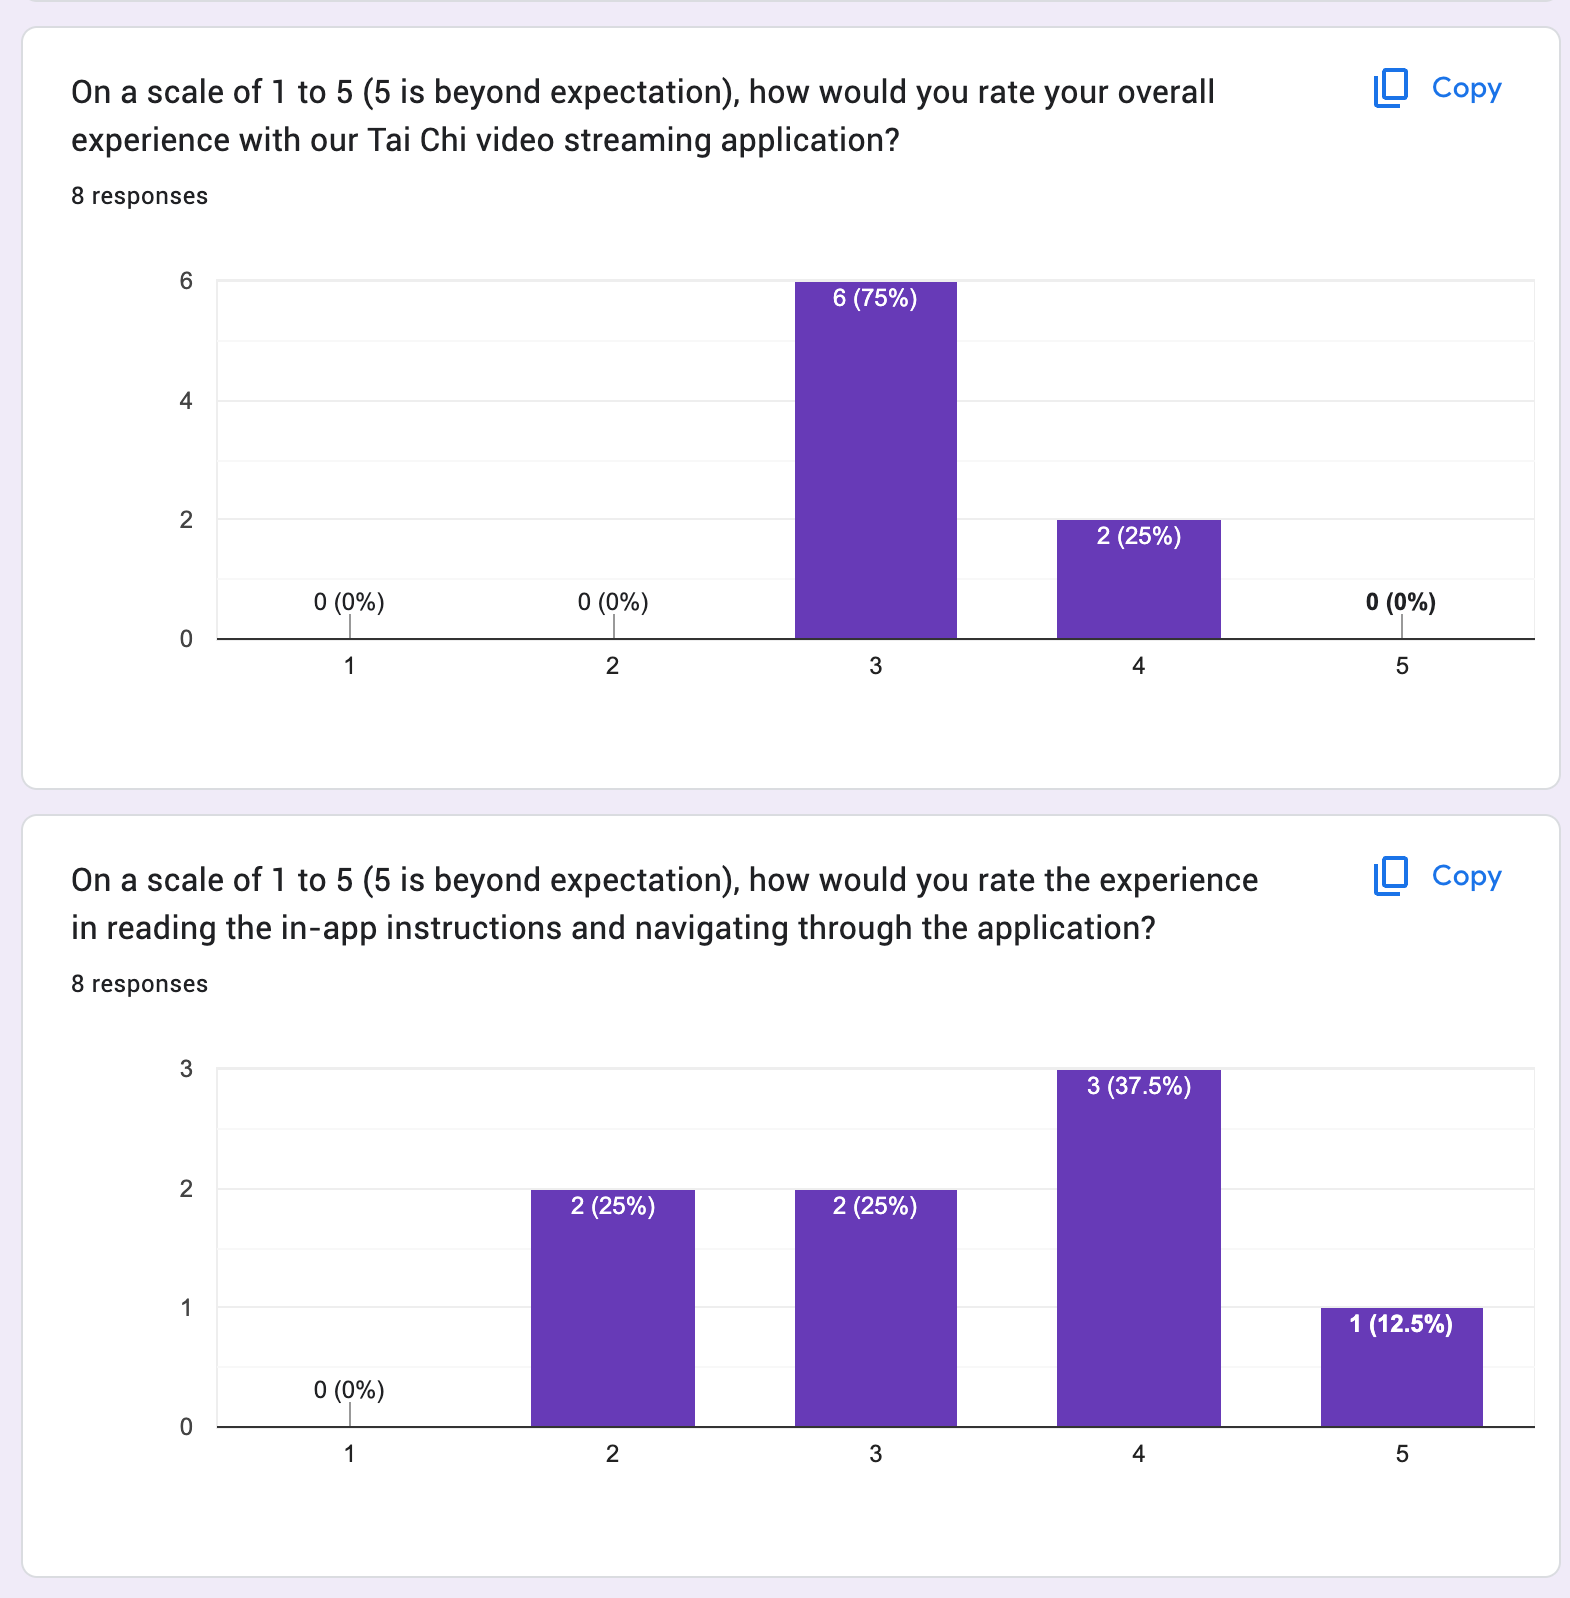
\includegraphics[width=1.0\linewidth]{surveyp1.png}
  \caption{Survey results part 1}
  \label{fig:surveyp1}
\end{figure}

\begin{figure}[h]
  \centering
  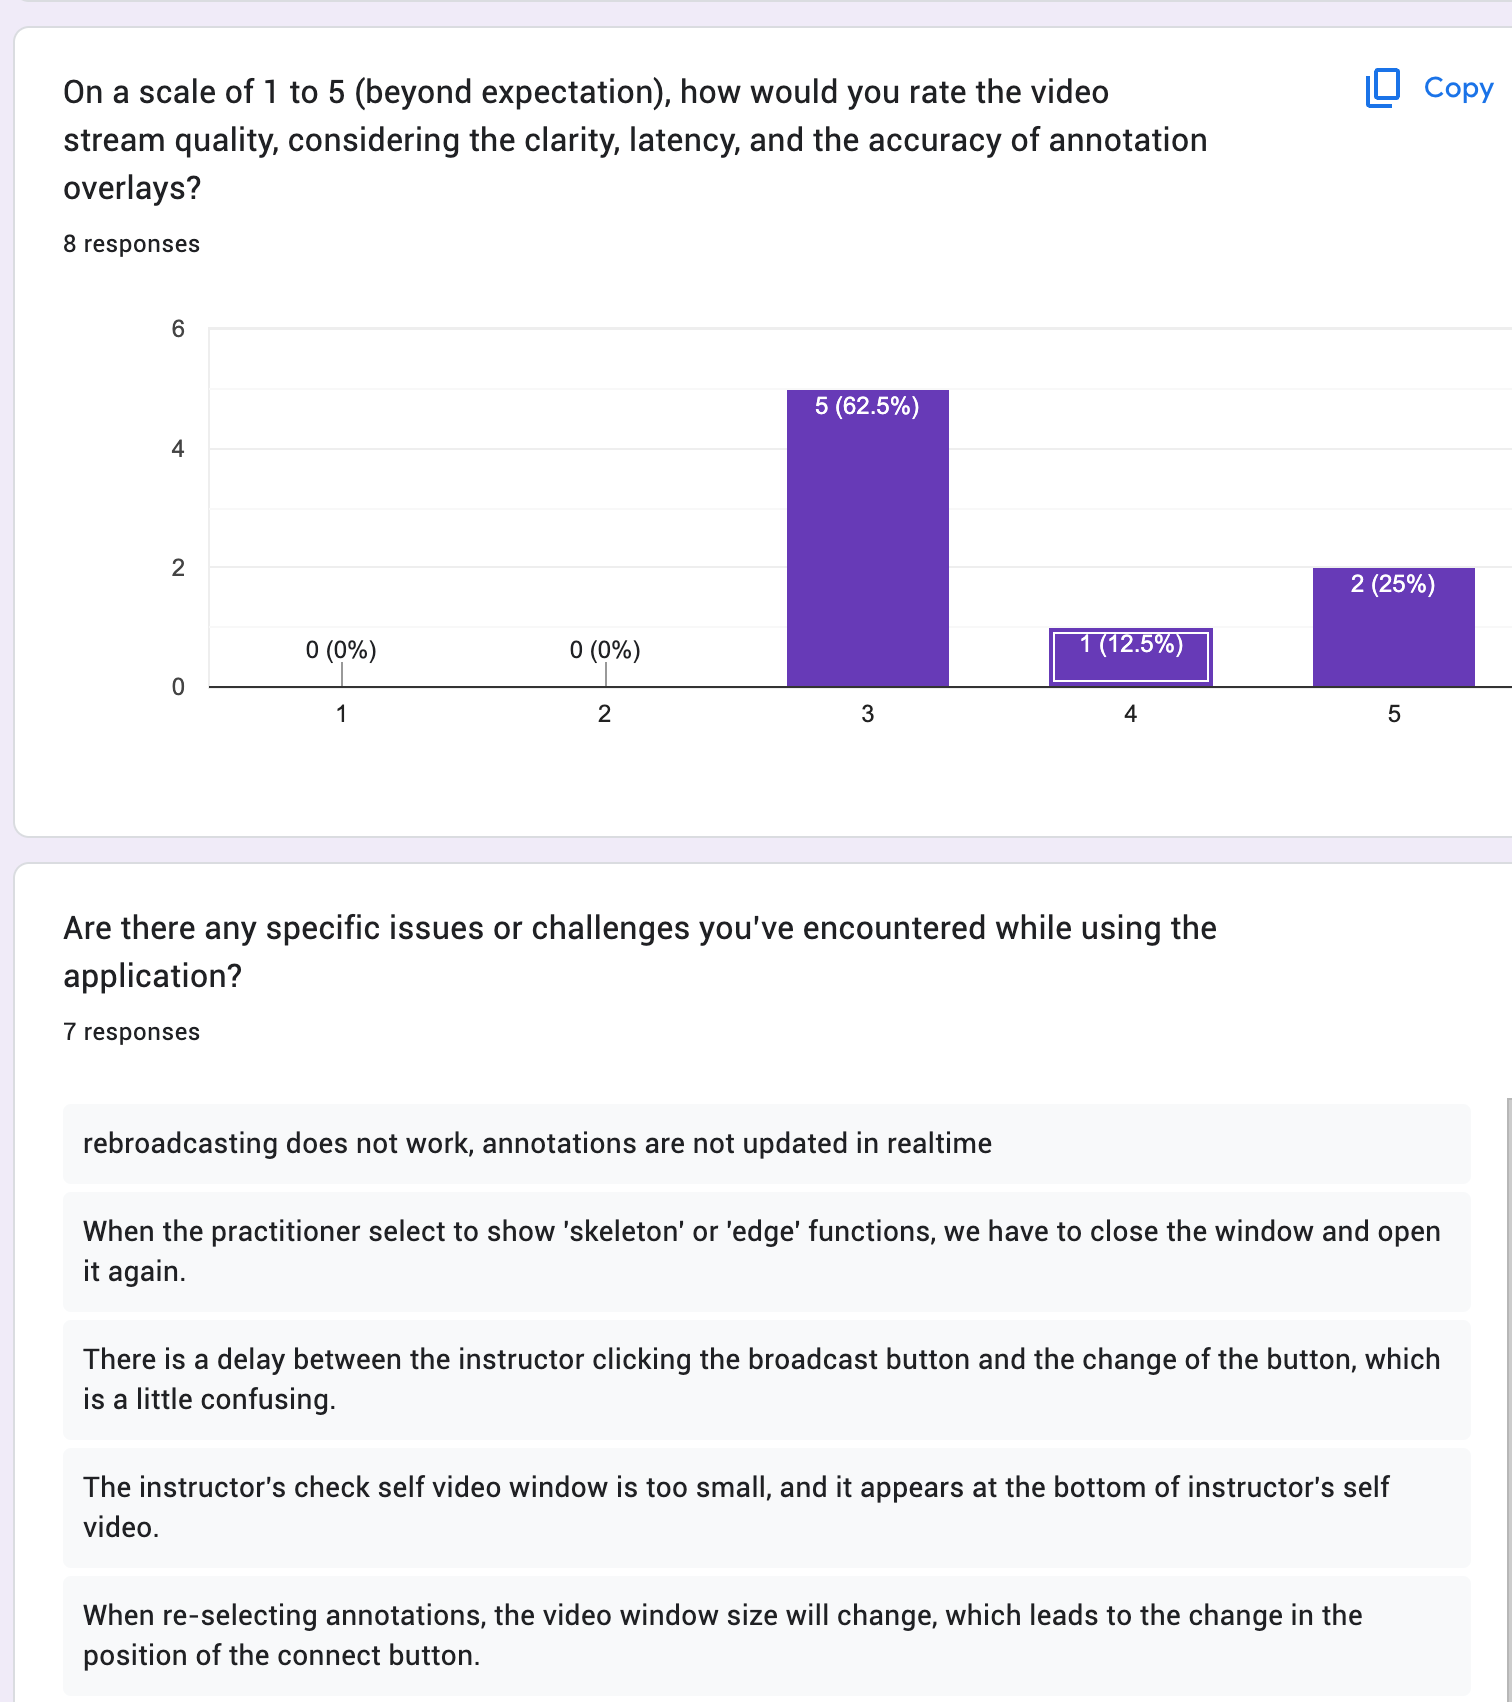
\includegraphics[width=1.0\linewidth]{surveyp2.png}
  \caption{Survey results part 2}
  \label{fig:surveyp2}
\end{figure}

\begin{figure}[h]
  \centering
  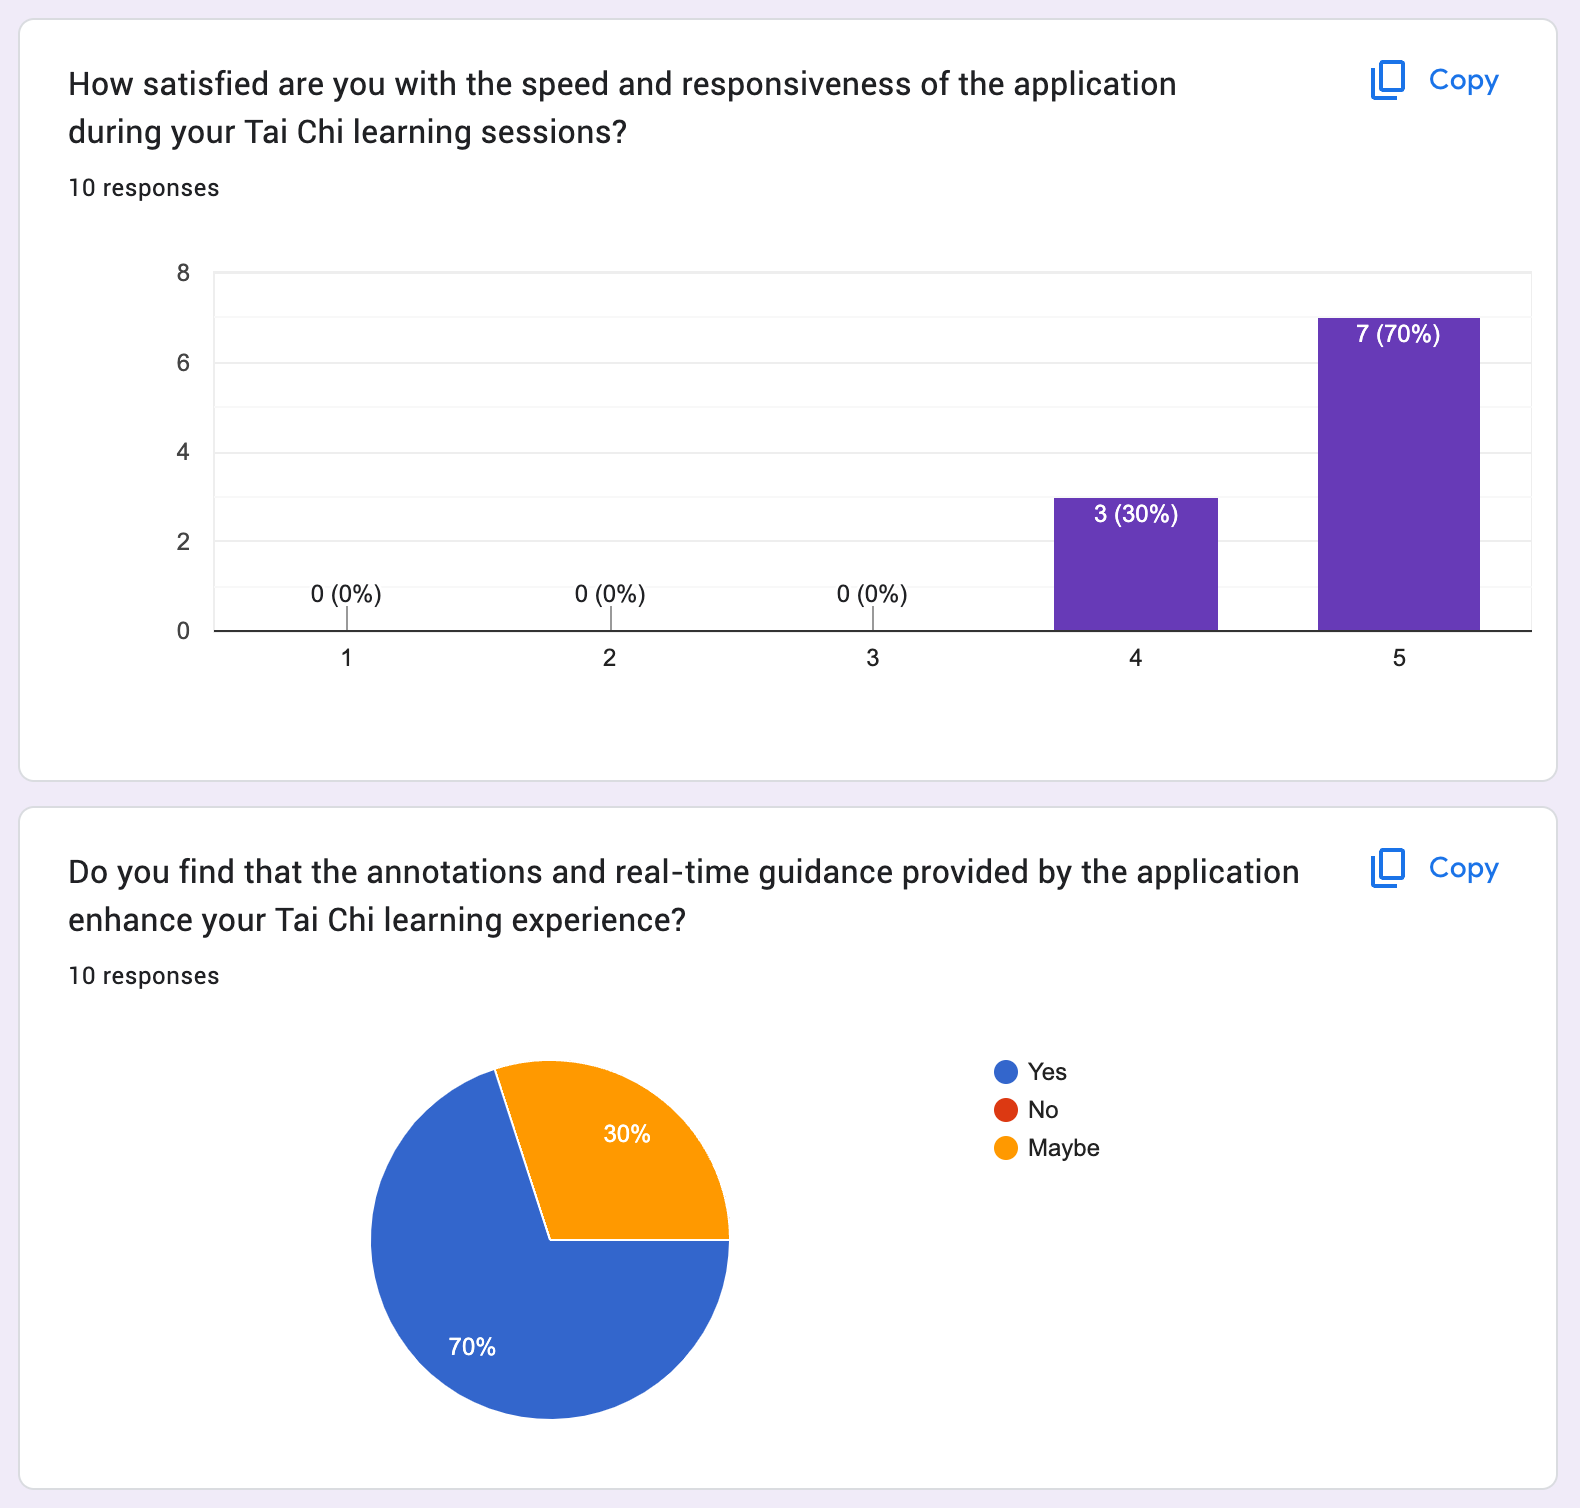
\includegraphics[width=1.0\linewidth]{surveyp3.png}
  \caption{Survey results part 3}
  \label{fig:surveyp3}
\end{figure}

\begin{figure}[h]
  \centering
  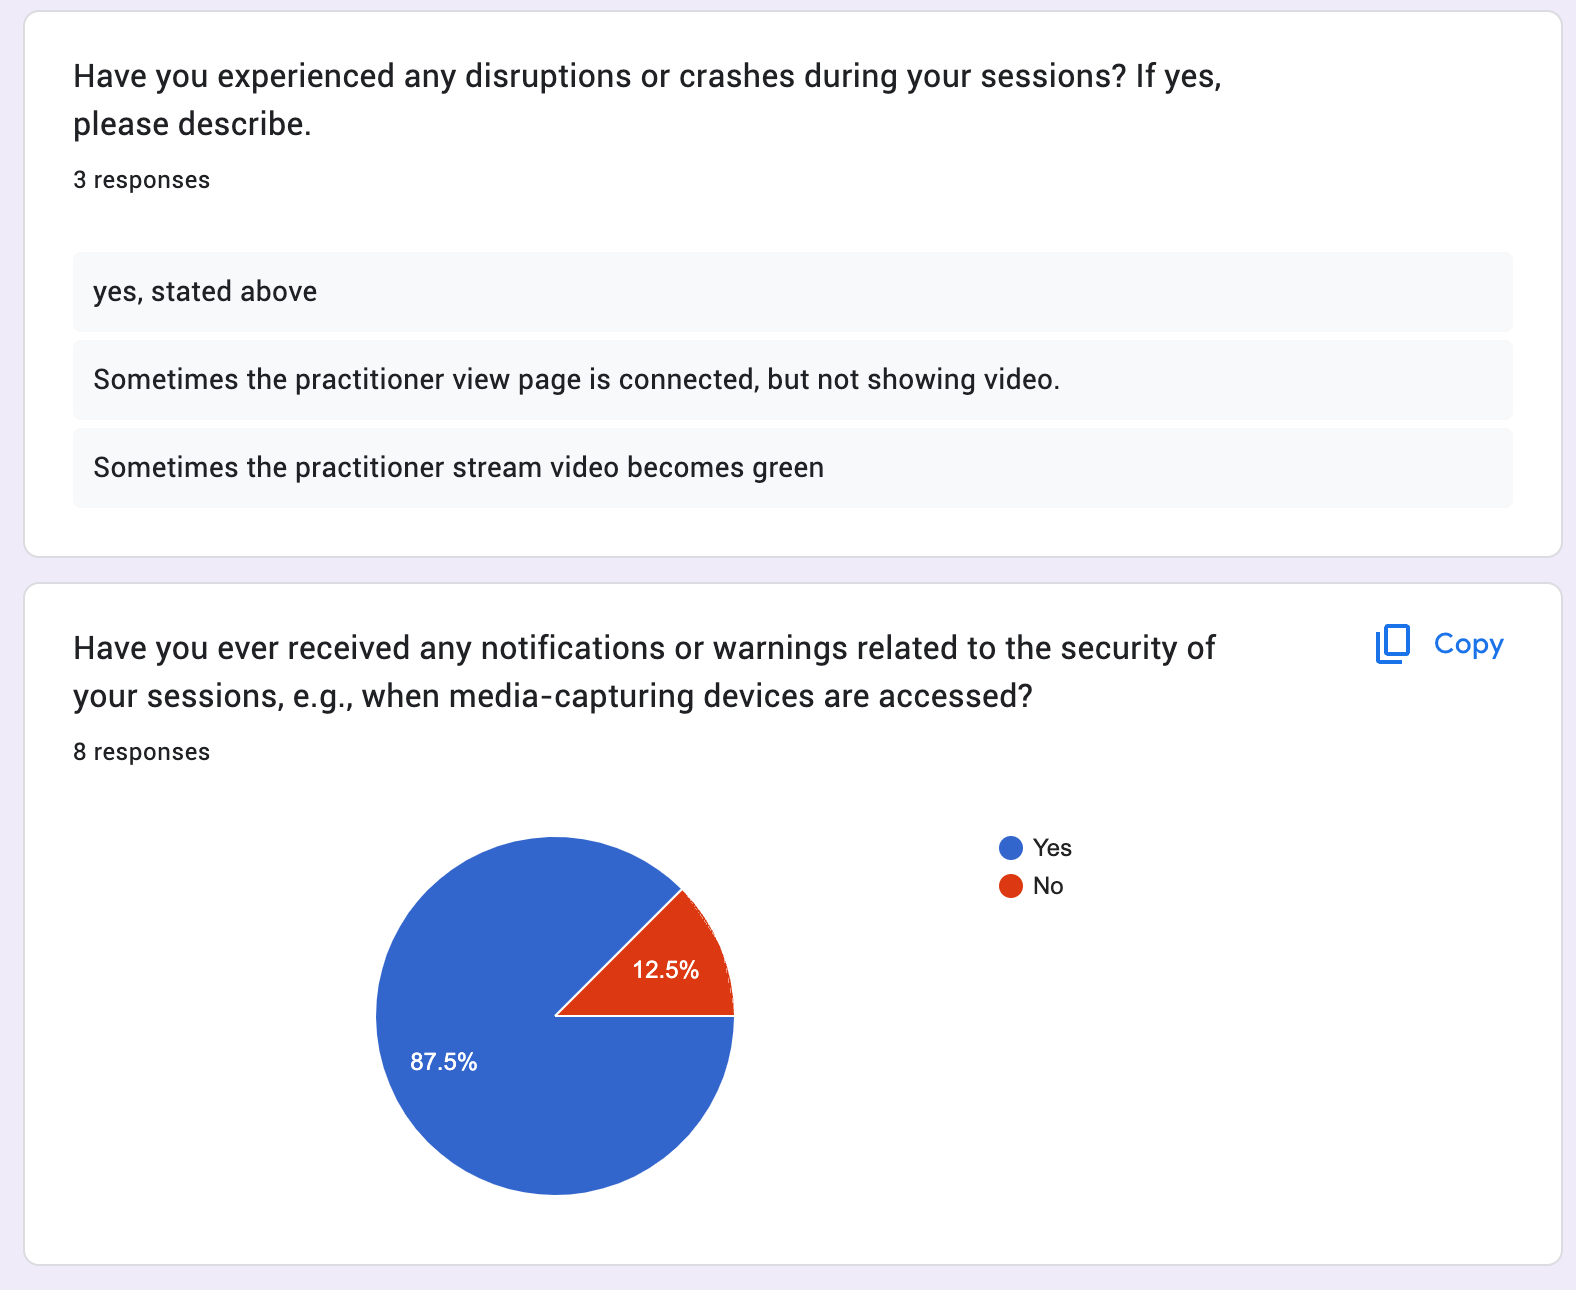
\includegraphics[width=1.0\linewidth]{surveyp4.png}
  \caption{Survey results part 4}
  \label{fig:surveyp4}
\end{figure}

\begin{figure}[h]
  \centering
  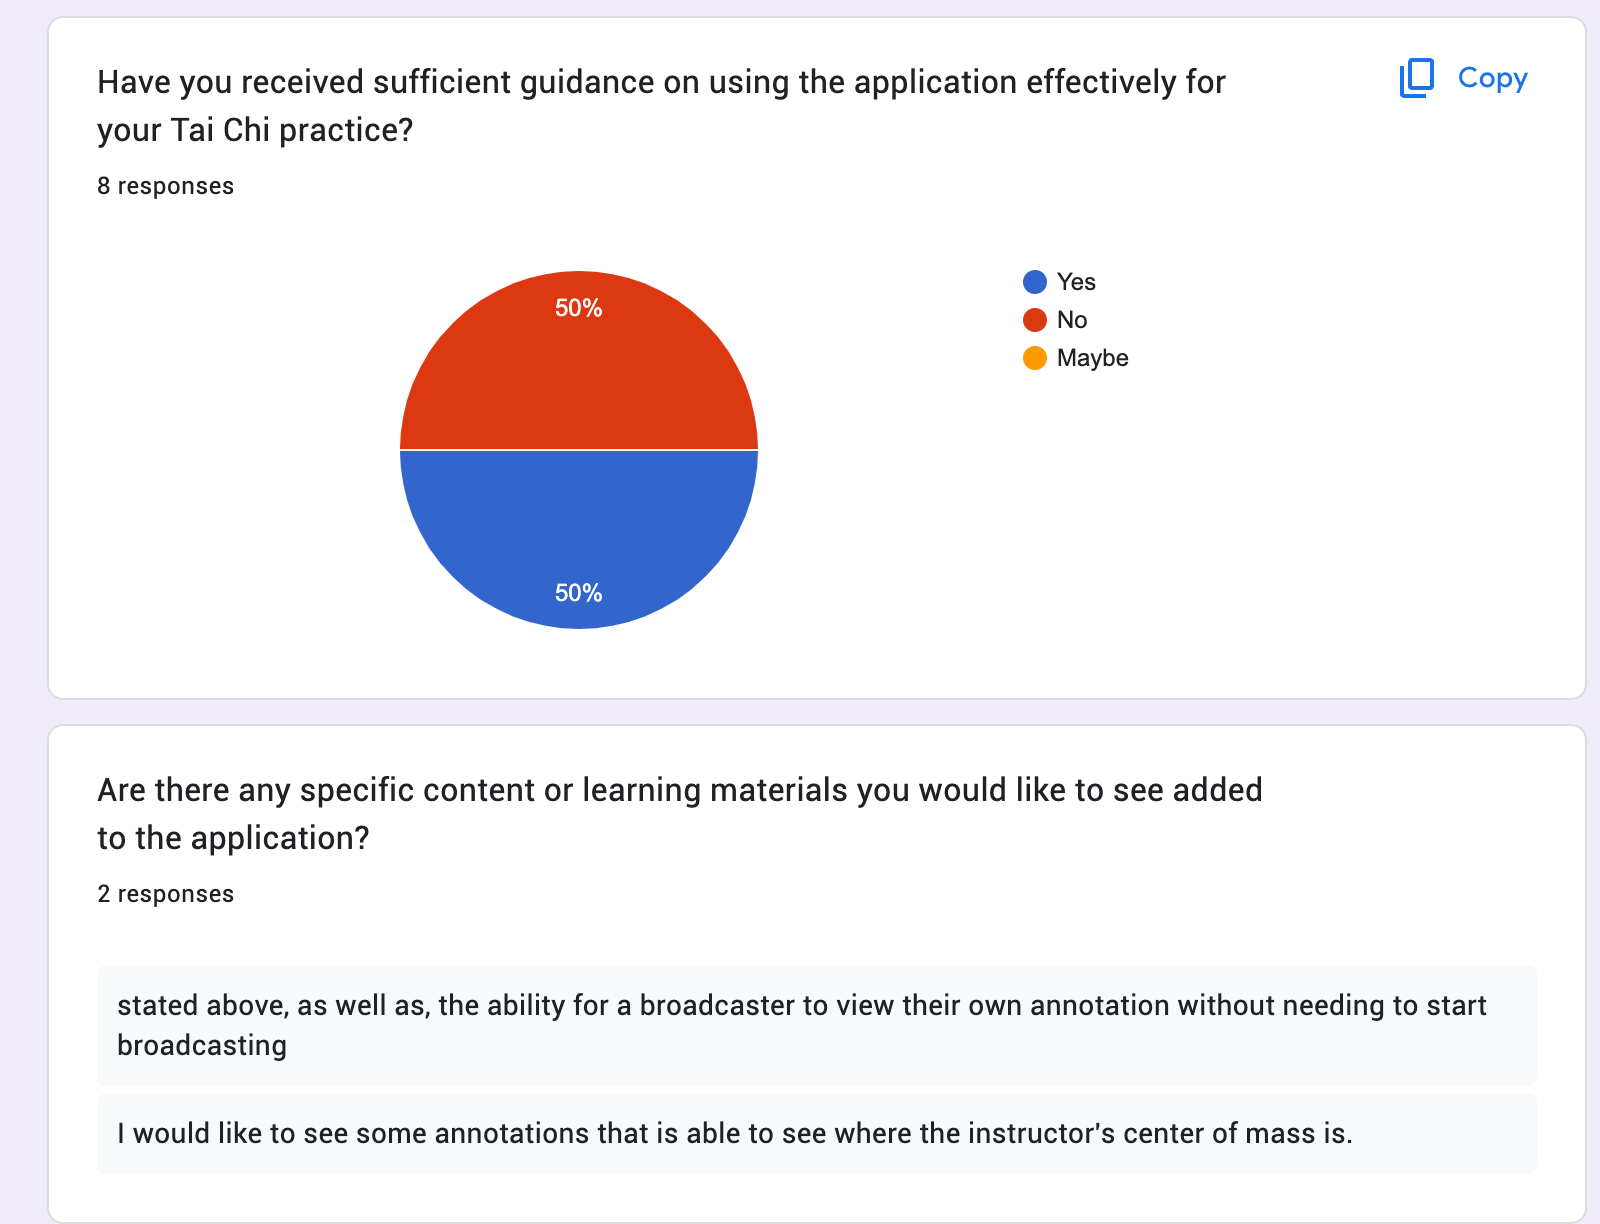
\includegraphics[width=1.0\linewidth]{surveyp5.png}
  \caption{Survey results part 5}
  \label{fig:surveyp5}
\end{figure}


\end{document}